
\section{Vybrané kartografické zobrazení}

Z hlediska zkreslení zobrazení rozlišujeme na:
\begin{enumerate}
\item konformní - stejnouhlá,
\item ekvidistantní - stejnodelná,
\item ekvivalentní - stejnoplochá,
\item kompenzační - vyrovnávací.
\end{enumerate}

Z pohledu k třídění zobrazovací plochy, pomocí které si můžeme představit vznik obrazu referernční lochy rozlišujeme:
\begin{enumerate}
\item zobrazení na kulovou plochu,
\item jednoduchá zobrazení (kuželová, válcová, azimutální),
\item nepravá zobrazení (pseudokonická, pseudocylindrická, pseudoazimutální),
\item polykónická,
\item polyederická, 
\item obecná.
\end{enumerate}
My popíšeme jenom vybrané jednoduchá zobrazení a to konrkétně válcová (UTM) a azitmální (stereografická projekce).

\subsection{Definice a některé vlastnosti vybraných kartografického zobrazení}

Kartografickým zobrazením je podle \cite{Buchar2002} vzájemné přiřazení polohy bodů na dvou různých referenčních plochách. V některých případech, kdy je možno vztah realizovat geometrickou cestou (promítaním), podle \cite{Buchar2002} budeme takové zobrazení nazývat projekcí neboli prospektivním zobrazením.

Zobrazení je jednoznačne matematicky definováno vtahem mezi souřadnicemi bodů na oboureferenčních plochách, kterému říkame zobrazovací rovnice. Například zobrazení elipsoidu do roviny budou zobrazovací rovnice v explicitním tvaru

\begin{equation}
X = f\left(\varphi, \lambda\right),
\end{equation}


\begin{equation}
Y = g\left(\varphi, \lambda\right),
\end{equation}
kde funkce \textit{f, g} v určitém místě považujeme za spojité, obecně na sobě mezávislé, diferencovatelné apod. Výjimky představují singulární body (např. póly), kde uvedená vlastnost není obecně splněna.

\subsubsection{Poznámky k jednoduchým zobrazením}
Pro naše účely nás budou zajímat jenom jednoduchá zobrazení. Jednoduchá zobrazní jsou taková zobrazení, pro něž je možno zapsat zobrazovací rovnice, podle nichž každá  z rovinných souřadníc (polárních nebo pravoúhlých) a výrazy pro zkreslení (zýávislé proměnné) se dají vyjádřit funkcemi pouze jedné souřadnice (nezávsilé proměnné) na referenční ploše. Důsledkem takové jednoduché volby je pak i jednoduchý obraz poledníků a rovnobežek, které jsou pak na mapě znázorněny jako svazek přímek čo osnova rovnoběřných přímek (u poledníku) a soustava rovnoběžných kružnic či osnova rovnoběžných přímek (u rovnoběžek). Jednoduchá zobrazení jsou ortogonální (viz \cite{Buchar2002}, str. 51).

\subsection{Poznámky k valcovým zobrazením}
Válcová zobrazení v normálni poloze mají tyto vlastnosti \cite{Buchar2002}:
\begin{enumerate}
\item rovník a rovnoběžky se zobrazují jako osnova rovnoběžných přímek,
\item obrazy poledníků tvoří osnovu přímek vzájemně stejně odlehlých rovnoběžných a kolmých na obrazy rovnoběžek,
\item obraz základního poledníku volíme jako osu Y, 
\item zobrazovací rovnica pro Y je veličina Y funkcí pouze $\left(\varphi\right)$.
\item do obrazou rovníku vkládame osu X (u souřadnícových systému používaných v geodézii je orientace opačná),
\item zobrazovací rovnica pro X je X lineární funkcí zeměpisné délky $\left(\lambda\right)$.
\end{enumerate}

Zkreslení v poledníku a rovnoběžce jsou:
\begin{equation}
m_{p} = \dfrac{dY}{M d\varphi}
\label{rov:zkresValPol}
\end{equation}

\begin{equation}
m_{r} = \dfrac{dX}{N \cos{\left(\varphi\right)d\lambda}} = \dfrac{a}{N\cos{\left(\varphi\right)}},
\label{rov:zkresValRov}
\end{equation}
kde \textit{M, N} jsou meridiánový a příčný poloměr křivosti, \textit{a} je hlavní poloosa meridiánové elipsy a $\varphi$ je zeměpisná šířka.

Protože poledník a rovnoběžka tvoří u válcových zobrazení hlavní paprsky, je pro konformitu jedinou a postačující podmínkou

$$m_{p} = m_{r},$$ 
a pri referenční ploše elipsoidické a nezkresleném rovníku bude pro dosazení \ref{rov:zkresValPol} a \ref{rov:zkresValRov}, platit:
\begin{equation}
\dfrac{dY}{M d\varphi} = \dfrac{a}{N\cos{\left(\varphi\right)}}.
\end{equation}
Po separaci proměnných dostaneme
\begin{equation}
dY = a\dfrac{M}{N\cos{\left(\varphi\right)}}d\varphi,
\label{rov:dY}
\end{equation}
kde na pravé straně rovnice se vyskytuje výraz pro tzv. izometrickou šířku.

Izometrická šířka \textit{q}, která je funkcí zeměpisné šířky $\varphi$, je definováná:
\begin{equation}
q = \int_{0}^{\varphi}\dfrac{M}{N\cos{\left(\varphi\right)}}d\varphi
\end{equation}
a po dosazení za \textit{M} a \textit{N} dostaneme
\begin{eqnarray}
q &=& \int_{0}^{\varphi} \dfrac{\left(1-e^{2}\right)}{\left(1-e^{2}\sin^{2}{\left(\varphi\right)}\right)\cos{\left(\varphi\right)}}d\varphi \\ \nonumber
  &=&\int_{0}^{\varphi}\dfrac{\left(1-e^{2}\sin^{2}{\left(\varphi\right)}-e^{2}\cos^{2}{\left(\varphi\right)}\right)d\varphi}{\left(1-e^{2}\sin^{2}{\left(\varphi\right)}\right)\cos{\left(\varphi\right)}} \\ \nonumber
  &=& \int_{0}^{\varphi}\dfrac{d\varphi}{\cos{\left(\varphi\right)}} - \int_{0}^{\varphi}\dfrac{e\cos{\left(\varphi\right)}d\varphi}{1-e^{2}\sin^{2}{\left(\varphi\right)}} \\ \nonumber
  &=& \ln\tan{\left(\dfrac{\varphi}{2} + \dfrac{\pi}{4}\right)} - e\int_{0}^{\varphi}\dfrac{d\left(e\sin{\left(\varphi\right)}\right)}{1-e^{2}\sin^{2}{\left(\varphi\right)}},
\end{eqnarray}
a po proložení $x = e\sin{\left(\varphi\right)}$ v posledním integrálu, z nehož plyne, že 
\begin{equation}
\int \dfrac{dx}{1-x^{2}} = \dfrac{1}{2}\ln{\left(\dfrac{1+x}{1-x}\right)} = \dfrac{1}{2}\ln{\left(\dfrac{1+e\sin{\left(\varphi\right)}}{1-e\sin{\left(\varphi\right)}}\right)}
\end{equation}
a pro izometrickou šířku pak platí
\begin{equation}
q = \ln{\left[\tan{\left(\dfrac{\varphi}{2}+\dfrac{\pi}{4}\right)}\left( \dfrac{1-e\sin{\left(\varphi\right)}}{1+e\sin{\left(\varphi\right)}} \right)^{\dfrac{e}{2}}\right]}.
\label{rov:izometricka}
\end{equation}
Po dosazení \ref{rov:izometricka} do \ref{rov:dY} dostaneme \cite{Buchar2002}, \cite{Snyder1987}:
\begin{equation}
Y = a\ln{\left[\tan{\left(\dfrac{\varphi}{2}+\dfrac{\pi}{4}\right)}\left( \dfrac{1-e\sin{\left(\varphi\right)}}{1+e\sin{\left(\varphi\right)}} \right)^{\dfrac{e}{2}}\right]}.
\label{rov:utmY}
\end{equation}
Protože \textit{X} je lineární funkce zeměpisné délky, pro vyjdřední souřadnice \textit{X} platí:
\begin{equation}
X = a\left(\lambda-\lambda_{0}\right).
\end{equation}

Inversní vzorec pro veličinu $\varphi$ v případě spětné transformace vyžaduje počítaní přes iterační proces a základní rovnice je definováná ve tvaru \cite{Snyder1987}

\begin{equation}
\varphi = \dfrac{\pi}{2} - 2 \tan^{-1}{\left\lbrace t \left[ \dfrac{1-e\sin{\left(\varphi\right)}}{1+e\sin{\left(\varphi\right)}} \right]^{\dfrac{e}{2}} \right\rbrace}, 
\end{equation}
kde
$$t = e^{\dfrac{-Y}{a}}$$
a iterační proces začína výpočtem
$$\varphi = \dfrac{\pi}{2}-2\tan^{-1}{\left(t\right)}$$
a pokračuje pokud není dosažení zvolená konvergenční hranice.

Inversní zeměpisná délka se vypočte podle rovnice:
\begin{equation}
\lambda = \dfrac{X}{a} + \lambda_{0}.
\end{equation} 

\subsubsection*{Konformní transversální válcové zobrazení}

Konformní transversální válcové zobrazení nazývané také Gaussovo (pro elipsoidickou referenční plochu) nebo transversální Mercatorovo, je specifické tím, že válec  se dotýka referenční koule (elipsoidu) podél základního poledníku, procházejíciho středem území. Kartografické poledníky a rovnoběžky se pak zobrazují jako zeměpisné polidníky a rovnoběžky v normálni poloze. 

Uplatnění našlo také konformní válcové zobrazení v obecné poloze (v literatuře Oblique Mercator Projection). Délkově zachovává zvolený kartografický rovník.

\subsubsection*{Universální transversální zobrazení v poledníkových pásech, zobrazení systému UTM}

V zobrazeních, v kterých má být užito v poloze jiné než normální, zobrazuje se najdřív elipsoid na kouli a pak terpve s koule na zobrazovací plochu, \cite{Buchar2002}. V případě Gauss (Gauss-Kr\"{u}gerova) zobrazení, elipsoid je zobrazován přímo do roviny, tedy bez zprostředkujíci koule a to tak, že meridiální pruhy stejné šířky se zobrazují samostatně. Určující podínkou je konformita a nezkreslený základní (střední) poledník pásu. 

\subsection{GEOD$\rightarrow$ UTM}

V knize \cite{Buchar2002} se uvádí podrobné odvození zobrazovacích rovníc. Z pohledu programatorského je možná výhodnějnší popsat algoritmus, který se nachádzí v knize \cite{Snyder1987} (vzorce platí pro elipsoid).

\begin{equation}
x = k_{0}N\left[A + \left(1-T+C\right)\dfrac{A}{6} + \left(5-18T+T^{2}+72C-58e^{'2}\right)\dfrac{A^{5}}{120}\right]
\end{equation}	

\begin{equation}
y = k_{0}\left\lbrace B - B_{0} + N \tan{\left(\varphi\right)\left[\dfrac{A^{2}}{2} + \left(5-T+9C+4C^{2}\right)\dfrac{A^{4}}{24}+\left(61-58T+T^{2}+600C-330e^{'2}\right)\dfrac{A^{6}}{720}\right]}\right\rbrace
\end{equation}

\begin{equation}
k = k_{0}\left[1+\left(1+C\right)\dfrac{A^{2}}{2}+\left(5-4T+42C+13C^{2}-28e^{'2}\right)\dfrac{A^{4}}{24} + \left(61-148T+16T^{2}\right)\dfrac{A^{6}}{720}\right],
\end{equation}
kde
\begin{itemize}
\item $k_{0}$ je multipliační konstanta $k_{0} = 0.9996$,
\item $e^{'2}$ je druhá excentricita rotačního eliposidu definováná také pomocí $e^{'2} = e^{2}/\left(1-e^{2}\right)$,
\item $N$ je příčný poloměr křivosti rotačního elipsoidu, 
\item $T = \tan^{2}{\left(\varphi\right)}$,
\item $C = e^{'2}\cos^{2}{\left(\varphi\right)}$,
\item $A = \left(\lambda-\lambda_{0}\right)\cos{\left(\varphi\right)}$ předpokladajíc, že $\lambda\ \text{a}\ \lambda_{0}$ jsou v radiánech,
\item $B$ je délka oblouku meridiánu od rovníku po $\varphi$. $B_{0} = B$ zpočtěná pro $\varphi_{0}$ a platí
\begin{eqnarray}\label{rov:B}
B = & a & \left(1 - \dfrac{e^{2}}{4} - \dfrac{3e^{4}}{64} - \dfrac{5e^{6}}{256} - \cdots \right)\varphi \\ \nonumber
    & -a & \left(\dfrac{3e^{2}}{8} + \dfrac{3e^{4}}{32} + \dfrac{45e^{6}}{1024} - \cdots\right)\sin{\left(2\varphi\right)}\\ \nonumber
    & +a & \left(\dfrac{15e^{4}}{256} + \dfrac{45e^{6}}{1024} + \cdots\right)\sin{\left(4\varphi\right)}\\ \nonumber
    & -a & \left(\dfrac{35e^{6}}{3072} + \cdots\right)\sin{\left(6\varphi\right)}\\ \nonumber
\end{eqnarray}
\item $\varphi$ je zeměpisná délka v radiánech.
\end{itemize}

Pokud $\varphi \pm \pi/2$, pak $x=0$, $y = k_{0}\left(B-B_{0}\right)$ a $k=k_{0}$.

Jednotlivé osi souřadníc jsou dané takto: Yová osa leži v obraze základnáho poledníku $\lambda_{0}$ a y roste směrem na sever. Xová osa je kolmá na Y a x roste směrem na východ. 

\subsection{UTM $\rightarrow$ GEOD}

Pro inversní vzroce podle \cite{Snyder1987}  platí:
\begin{eqnarray}
\varphi = \varphi_{1} &-& G\left[\dfrac{D^{2}}{2}-\left(5+3T_{1}+10C_{1}-4C_{1}^{2}-9e^{'2}\right)\dfrac{D^{4}}{24}\right] \\ \nonumber
                      &-& G\left[\left(61+90T_{1}+298C_{1}+45T_{1}^{2}-252e^{'2}-3C_{1}^{2}\right)\dfrac{D^{6}}{720}\right], 
                      \label{rov:invPhi}
\end{eqnarray}

\begin{eqnarray}
\lambda = \lambda_{0} + \dfrac{D-\left(1+2T_{1}+C_{1}\right)\dfrac{D^{3}}{6} + \left(5-2C_{1}+28T_{1}-3C_{1}^{2}+8e^{'2} + 24T_{1}^{2}\right)\dfrac{D^{5}}{120}}{\cos{\left(\varphi_{1}\right)}},
\label{rov:invLam}
\end{eqnarray}
kde

\begin{itemize}
\item $G = \left(\dfrac{N_{1}\tan{\left(\varphi_{1}\right)}}{R_{1}}\right)$
\item $\varphi_{1}$ je zeměpisná šířka charakteristická pro centrální meridián a která ma stejnou \textit{y} souřadnici jako bod, kterého polární sořadnice jsou $\left(\varphi, \lambda\right)$ 
\begin{eqnarray} \nonumber
\varphi_{1} = \mu &+& \left( \dfrac{3e_{1}}{2} - \dfrac{27e_{1}^{3}}{32} + \cdots \right)\sin{2\mu} \\ \nonumber
                  &+& \left( \dfrac{21e_{1}}{16} - \dfrac{55e_{1}^{4}}{32} + \cdots \right)\sin{4\mu} \\ \nonumber
                  &+& \left( \dfrac{151e_{1}^{3}}{96} + \cdots \right)\sin{6\mu} \\ \nonumber
                  &+& \left( \dfrac{1097e_{1}^{4}}{512} - \cdots \right)\sin{8\mu} \nonumber
\end{eqnarray}
\item $
e_{1} = \dfrac{1 - \sqrt{1-e^{2}}}{1 + \sqrt{1-e^{2}}}
$
\item $\mu = \dfrac{B}{a\left(1-\dfrac{e^{2}}{4} - \dfrac{3e^{4}}{64} - \dfrac{5e^{6}}{256} - \cdots\right)} 
$
\item $B_{0}$ je spočtená pomocí rovnice \ref{rov:B} pro vstupní $\varphi_{0}$,
\item $B = B_{0} + \dfrac{y}{k_{0}}$,
\item $e^{'2} = \dfrac{e^{2}}{\left(1-e^{2}\right)}$,
\item $C_{1} = e^{'2}\cos^{2}{\left(\varphi_{1}\right)}$,
\item $T_{1} = \tan^{2}{\left(\varphi_{1}\right)}$,
\item $N_{1} = \dfrac{a}{\sqrt{\left(1-e^{2}\sin^{2}{\left(\varphi_{1}\right)}\right)}}$,
\item $R_{1} = \dfrac{a\left(1-e^{2}\right)}{\left(1-e^{2}\sin^{2}{\left(\varphi_{1}\right)}\right)^{3/2}}$,
\item $D = \dfrac{x}{N_{1}k_{0}}$.
\end{itemize}

\subsubsection*{Meridiánová konvergence}
Meridiánová konvergence je podle \cite{webVUGTK} úhel určitém bodu referenční plochy mezi tečnami k místnímu poledníku a ke křivce rovnoběžné se základním poledníkem; může být elipsoidická meridiánová konvergence, sférická meridiánová konvergence a rovinná meridiánová konvergence.

V knize \cite{Buchar2002}, vzorec pro výpočet meridiánové konvergence $\gamma$ je (bez odvození)
\begin{eqnarray}
\tan{\left(\gamma\right)} &=& \lambda\sin{\left(\varphi\right)} + \dfrac{\lambda^{3}}{3}\sin{\left(\varphi\right)} \cos^{2}{\left(\varphi\right)}\left(1+\tan^{2}{\left(\varphi\right)} + 3\eta^{2} + 2\eta^{4} \right)  \\ \nonumber
                         &+&\dfrac{\lambda^{5}}{15}\sin{\left(\varphi\right)} \cos^{4}{\left(\varphi\right)}\left(2+4\tan^{2}{\left(\varphi\right)} +2\tan^{4}{\left(\varphi\right)} \right) + \cdots, \nonumber
\end{eqnarray}
kde $\eta^{2} = \dfrac{e^{2}\cos^{2}{\left(\varphi\right)}}{1-e^{2}}$.

\subsubsection*{Délkové zkreslení}
Délkové zkreslení je funkcií zeměpisných souřadníc a pre jeho výpočet platí \cite{Buchar2002}:
\begin{equation}
m = 1+\dfrac{\lambda}{2}\cos^{2}{\left(\varphi\right)}.
\end{equation}
Chceme-li délkové zkreslení zpočíst z pravouhlých souřadníc, pak vzorec pre výpočet je tento:
\begin{equation}
m = 1+\dfrac{y^{2}}{2R^{2}} + \dfrac{y^{4}}{24R^{4}} + \cdots,
\end{equation}
avšak $R = \sqrt{MN}$ je funkcí zeměpisné šířky $\varphi$.



\subsection{Poznámky k azimutálním zobrazením}

Azimutální zobrazení si můžeme představit tak, že obraz referenčního tělesa vzniká již přímo v rovině \cite{Buchar2002}, str. 99. V tomto zobrazení je rovina kolmá ke spojnici kartografického pólu se sředem referenční koule (pozor na projekci z elipsoidu). Nasledujíci text se týka odvození zobrazení vývozené z referenční koule. V knize \cite{Snyder1987} se diskutuje algoritmus respektíve vzorce platné pro elipsoid.

Z azimutálniho zobrazení jsou známá některé vlastnosti, například:

\begin{itemize}
\item Obrazem poledníků je svazek přímek s vrcholem v kartografickém pólu a které svírají stejné úhly jako na kouli.
\item Základní poledník se zobrazí jako osa X.
\item Obrazem rovnoběžek jsou kružnice se středem v kartografickém pólu. Poloměr těchto rovnoběžek závisí na kartografické šiřce.
\end{itemize} 

Zobrazovací rovnice jsou:
\begin{equation}
\rho = f\left(\psi\right),
\end{equation}
kde $\psi = 90^{\circ}-\varphi$, kde v tomto případe $\varphi$ je kartografická šířka (odvozená na kouli a ne na elipsoidu).
\begin{equation}
\varepsilon = \lambda,
\end{equation}
kde $\lambda$ v tomto případe reprezentuje kartografickou délku.

Funkci \textit{f} v případě první zobrazovací rovnice definujeme na základě požadávků, nejčastěji z ekvidistance, ekvivalence či konfomity. Nás bude zajímat konformní zobrazení, protože stereografická projekce zachováva konformitu úhlů.

V azimutálním zobrazení můžeme zavést pravouhlou rovinnou soustavu, kde pravoúhlé souřadnice X, Y získame transformací polárních souřadníc na pravouhlé souřadnice. Počátek takéto souřadnicové soustavy je potom někdy vhodné pomocí aditačních konstant přesunout do libovolného místa vzhledem k středu zobrazovaného území a to tak, aby souřadnice v tomto území měly kladnou hodnotu.

K transformaci polárních souřadníc do soustavy pravouhlých souřadnic použijeme výrazy:
\begin{equation}
X = \rho \cos{\left(\varepsilon\right)},
\end{equation}

\begin{equation}
Y = \rho \sin{\left(\varepsilon\right)},
\end{equation}
resp. pro inversní případ platí:
\begin{equation}
\rho = \sqrt{X^{2} + Y^{2}},
\end{equation}
a
\begin{equation}
\varepsilon = \tan^{-1}{\left(\dfrac{Y}{X}\right)}.
\end{equation}

Jak už bylo nastíněno, nás bude zajímat konformní zobrazení. Pro  konformní azimutální zobrazení je jedninou a postačující podmínkou

\begin{equation}
\dfrac{d\rho}{Rd\psi} = \dfrac{\rho}{R\sin{\left(\psi\right)}}.
\end{equation} 
Po separaci proměnných 
\begin{equation}
\dfrac{d\rho}{\rho} = \dfrac{d\psi}{\sin{\left(\psi\right)}}
\end{equation}
a po integraci dostaneme
\begin{equation}
\ln{\left(\rho\right)} = \ln{\left(\tan{\left(\dfrac{\psi}{2}\right)}\right)} + \ln{\left(C\right)},
\end{equation}
kde \textit{C} je libovolná integrační konstanta a z poslední rovnice plyne, že
\begin{equation}
\rho = C\tan{\left(\dfrac{\psi}{2}\right)}.
\end{equation}
Pokud zavedeme podmínku, aby pro střed mapy (pro pól) platilo $m = 1$, pak (bez odvození - viz \cite{Buchar2002}), $C = 2R$, takže zobrazovací rovnice jsou
\begin{equation}
\rho = 2R\tan{\left(\dfrac{\psi}{2}\right)}
\end{equation}
a
\begin{equation}
\varepsilon = \lambda.
\end{equation}
Výraz pro zkreslení $m$ je
\begin{equation}
m = \dfrac{1}{\cos{\left(\dfrac{\psi}{2}\right)}}.
\end{equation}

Pokud chceme stanovit v pólu konkrétní délkové zkreslení různe od jedné, je možné, podobně jako v případe UTM zobrazení, zavést multiplikační konstantu, jejíž velkost udává délkové zkreslení v pólu. Platí
\begin{equation}
C = k2R.
\end{equation}

Vedle konformity má zobrazení důležitou vlastnost, že každá kružnice na referenční ploše kulové se zobrazuje opět jako kružnice. Tedy obrazy geografické sítě se skládá ze samých kružnic respektíve přímek (kružnice s nulovou křivostí).

Výraz pro délkové zrekslení je možné vyjádřit i za použití rovinných souřadníc a to v tvaru
\begin{equation}
m = 1+\dfrac{X^{2}+Y^{2}}{4R^{2}}, 
\end{equation}
kde \textit{R} je poloměr koule.

\newpage
\subsection{GEOD $\rightarrow$ STEREO}

Azimutální (geometrické) projekce vznikají promítnutím povrchu referenční koule o poloměru \textit{R} z libovolného bodu $K_{c}$ na rovinu $\pi$, kolmou ke spojnici středu promítaní $K_{c}$ se středem kolue \textit{C}. Podle předchozího obrázku, který znázorňuje osový řez rovinou promítacího paprsku bodu P, je obraz bodu $P^{'}$ určen v rovině $\pi$ polárnimi souřadnicemi $\rho, \varepsilon$.

\begin{figure}[ht!]
\begin{center}

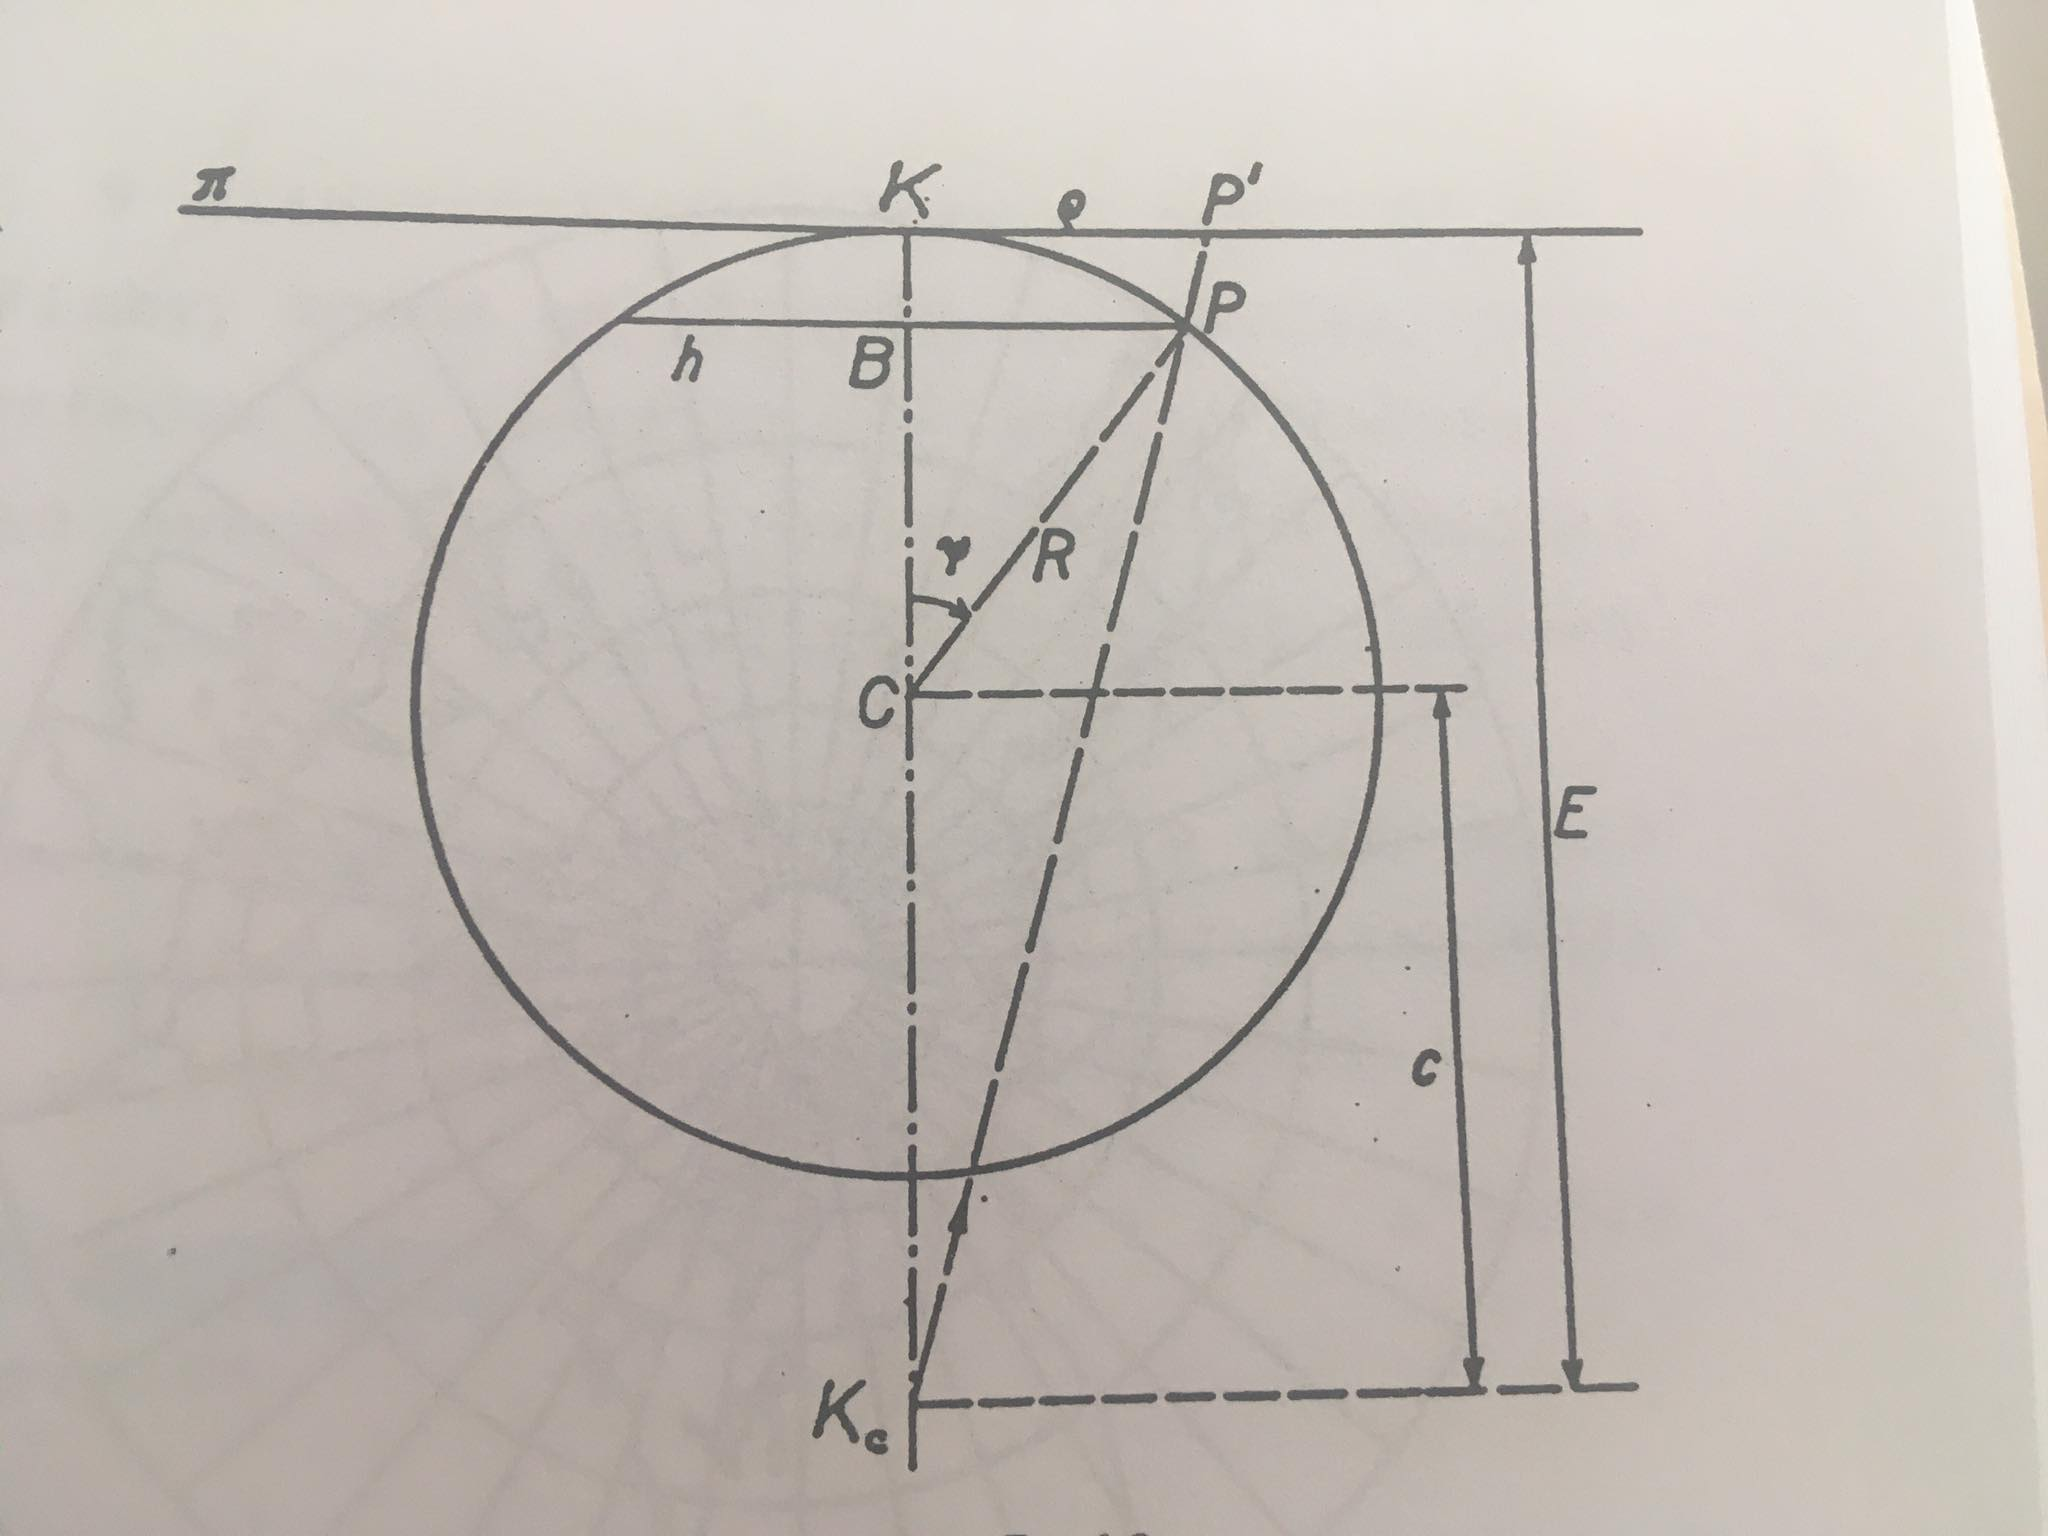
\includegraphics[width=0.5\textwidth]{FIG/azimProj.jpg}
\caption{Geometrická azimutální projekce. Obrázek je převzat z \cite{Buchar2002}.}
\label{fig:azimProj}
\end{center}
\end{figure}

Z obrázku plyne táto nerovnost
\begin{equation}
\dfrac{\rho}{R\sin{\left(\psi\right)}} = \dfrac{E}{c+R\cos{\left(\psi\right)}},
\end{equation}
kde $E = K_{c}K$ a $c = K_{c}C$, kde \textit{C} je střed koule. Takže zobrazovací rovnice azimutálních zobrazení budou

\begin{equation}
\rho = \dfrac{RE\sin{\left(\psi\right)}}{c+R\cos{\left(\psi\right)}}
\end{equation}
a
\begin{equation}
\varepsilon = \lambda.
\end{equation}

Vztahy pro výpočet pravouhlých souřadníc transformované z polárních souřadníc, resp. přímo ze zeměpisných souřadníc jsou (porovnej s \cite{stereoWolf} anebo \cite{Thomas1977},  kde je přehozené značení souřadnicových os).
\begin{equation}
X = \dfrac{RE\left(-\cos{\left(\varphi_{K}\right)}\sin{\left(\varphi\right)}+\sin{\left(\varphi_{K}\right)}\cos{\left(\varphi\right)}\cos{\left(\Delta\lambda\right)}\right)}{c+R\left( \sin{\left(\varphi_{K}\right)}\sin{\left(\varphi\right)}+\cos{\left(\varphi_{K}\right)}\cos{\left(\varphi\right)}\cos{\left(\Delta\lambda\right)} \right)},
\end{equation}
a
\begin{equation}
Y = \dfrac{RE\left(\cos{\left(\varphi\right)}\sin{\left(\Delta\lambda\right)}\right)}{c+R\left( \sin{\left(\varphi_{K}\right)}\sin{\left(\varphi\right)}+\cos{\left(\varphi_{K}\right)}\cos{\left(\varphi\right)}\cos{\left(\Delta\lambda\right)} \right)},
\end{equation}
kde $\Delta\lambda = \left(\lambda - \lambda_{K}\right)$.

Rovnice platí pro všechny azimutální projekce. Jedina neznáma konstanta \textit{c} rozhoduje výběr projekce zo sady případů, z nichž užívané jsou:
\begin{itemize}
\item gnomická projekce, při $c = 0$;
\item {\textbf{stereografická projekce}}, při $c = R$;
\item externí projekce, při $c > R$;
\item ortografická projekce, při $c = \infty$.
\end{itemize} 

Poznamenajme, že rovnice stereografické projece, která zobrazuje referenční těleso elipsoid do roviny jsou obsahem knihy \cite{Snyder1987}.

\subsection{STEREO $\rightarrow$ GEOD}.

Inverzní vzorce pro odhad zeměpisných souřadníc z pravouhlých rovinných souřadníc jsou \cite{Thomas1977} anebo \cite{stereoWolf} (pozor na přehozené značení souřadnicových os):

\begin{equation}
\varphi = \sin^{-1}{\left(\cos{\left(c\right)}\sin{\left(\varphi_{K}\right)}\dfrac{Y\sin{\left(c\right)}\cos{\left(\varphi_{K}\right)}}{\rho}\right)},
\end{equation}
a
\begin{equation}
\lambda = \lambda_{0} +  \tan^{-1}{\left(\dfrac{X\sin{\left(c\right)}}{\rho\cos{\left(\varphi_{K}\right)}\cos{\left(c\right)}-Y\sin{\left(\varphi_{K}\right)}\sin{\left(c\right)}}\right)},
\end{equation}
kde
\begin{equation}
\rho = \sqrt{X^{2} + Y^{2}}
\end{equation}
a
\begin{equation}
c = 2\tan^{-1}{\left(\dfrac{\rho}{2R}\right)}.
\end{equation}

